\chapter{Related Work}
\section{Reinforced Signal Control (RESCO)}
In this section, we review related work in the field of traffic signal control, with a focus on the Reinforced Signal Control (RESCO) toolkit, which serves as a baseline for my research.

The RESCO toolkit is a standard Reinforcement Learning (RL) traffic signal control testbed designed to achieve several key objectives:

\begin{enumerate}
    \item Provide benchmark single and multi-agent signal control tasks based on well-established traffic scenarios.
    \item Offer an OpenAI GYM interface within the testbed environment to facilitate the deployment of state-of-the-art RL algorithms.
    \item Deliver a standardized implementation of state-of-the-art RL-based signal control algorithms.
\end{enumerate}

RESCO is open-source and freely available under the GNU General Public License 3. It is built on top of SUMO-RL \cite{alegre2019sumo-rl} and can be accessed on GitHub at \url{github.com/Pi-Star-Lab/RESCO}. The embedded traffic scenarios within RESCO have their own licensing, with Cologne-based scenarios under Creative Commons BY-NC-SA and Ingolstadt-based scenarios under the GNU General Public License 3.

\subsection{State and Action Space}

RESCO accommodates a wide range of sensing assumptions, including advanced sensing capabilities \cite{codeca2018monaco}. Users can select subsets of state features based on specific sensing assumptions. Features include information such as stopped vehicles' queue length, the number of approaching vehicles, total waiting time for stopped vehicles, and more, at the level of state, intersection, and lane. Additionally, users can define the effective sensing distance during initialization.

The action space in RESCO encompasses sets of non-conflicting phase combinations, following the methodology described in Section 2.2 of the RESCO documentation \cite{codeca2018monaco}. By default, actions are chosen for the next 10 seconds of simulation, with the first 3 seconds reserved for yellow signals, if necessary.

\subsection{Reward Metrics}

RESCO offers flexibility in terms of reward metrics. Users can designate any of the reward metrics defined in Section 2.2 of the RESCO documentation\cite{codeca2018monaco} or create custom weighted combinations of these metrics. When initializing a control task, users can pass a weight vector that assigns weights to different metrics in the reward function. These weights correspond to various aspects, such as system travel time, signal-induced delays, total waiting time at intersections, average queue length, and traffic pressure.

\subsection{Benchmark Control Tasks}

The signal control benchmark tasks in RESCO are based on two well-established SUMO scenarios: "TAPAS Cologne" and "InTAS" \cite{pham2013learning, lobo2020intas}. These scenarios represent traffic within real-world cities, namely, Cologne and Ingolstadt in Germany. They include road network layouts and calibrated demands, making them suitable for comprehensive evaluation. RESCO defines three benchmark control tasks for each traffic scenario:

\begin{enumerate}
    \item Controlling a single main intersection.
    \item Coordinated control of multiple intersections along an arterial corridor.
    \item Coordinated control of multiple intersections within a congested area (downtown).
\end{enumerate}

\subsection{Benchmark Algorithms}

RESCO provides three baseline controllers and several RL-based controllers for comparative evaluation:

\begin{enumerate}
    \item \textbf{Baseline Controllers}:
    \begin{enumerate}
        \item Fixed-time (Pre-timed) control, where phase combinations are enabled for fixed durations following predefined cycles, that was recorded physically from the real-world traffic signal controller.
        \item Max-pressure control, which selects the phase combination with the maximum joint pressure. \cite{chen2020toward}
        \item Greedy control, which chooses the phase combination with the maximum joint queue length and approaching vehicle count.\cite{ma2020feudal}
    \end{enumerate}
    
    \item \textbf{RL Controllers}:
    \begin{enumerate}
        \item IDQN (Independent DQN agents), employing convolutional layers for lane aggregation\cite{ault2020learning}.
        \item IPPO, which utilizes a deep neural network similar to IDQN\cite{ault2020learning}.
        \item MPLight, based on the FRAP open-source implementation, ChainerRL DQN\cite{ChainerRL}, and pressure sensing\cite{zheng2019learning}.
        \item Extended MPLight (MPLight*), an enhanced version of MPLight with additional sensing information.
        \item FMA2C, built on top of the MA2C open-source implementation\cite{chu2019multi}.
    \end{enumerate}
\end{enumerate}

In each of the RL-based controllers, specific learning algorithms and hyperparameters are applied, allowing for a comprehensive evaluation of their performance \cite{ault2020learning, chen2020toward, chu2019multi, ma2020feudal, zheng2019learning}.

In the case of IDQN, IPPO, and MPLight, the implementation of the learning algorithm is invoked directly from the ChainerRL \cite{ChainerRL} and the Preferred RL \cite{ChainerRL} libraries that is successor of ChainerRL, and customized to align with my specific map and requirements.

\section{Reinforcement-Learning-Light (RLight)}
Adaptive Traffic Signal Control (ATSC) is a critical aspect of modern transportation systems, with the primary goal of enhancing traffic flow, reducing travel times, and mitigating CO2 emissions \cite{zhao2011computational}. Traditional methods of traffic signal control often rely on manually crafted rules that cater to specific traffic scenarios. However, recent advancements in traffic data collection and optimization techniques suggest new possibilities \cite{wei2019survey}.

In recent years, the integration of deep learning and reinforcement learning (RL) has shown remarkable success in solving complex tasks, often achieving super-human performance in various domains \cite{hernandez2019survey, mnih2015human, silver2018general}. This success raises the question of whether deep RL can bring similar benefits to ATSC.

Yet, ATSC poses a unique challenge from an RL perspective. Unlike many RL applications where the environment naturally maps to a Markov Decision Process (MDP), ATSC lacks a clear source of raw data and rewards, and it doesn't have a fixed set of actions or action rates. The quality of the MDP representation plays a crucial role in the success of ATSC \cite{zheng2019diagnosing}.

Previous models that aim to provide agents with comprehensive information often result in unnecessary complexity that hampers performance \cite{zheng2019diagnosing}. In contrast, Light-Intellight (LIT) \cite{zheng2019diagnosing} proposes a minimal set of features based on a uniform traffic distribution, demonstrating effective performance. However, urban traffic often exhibits non-uniform, clustered patterns, as depicted in Figure \ref{fig:atsc_clustering}. Surprisingly, prior work has not specifically tailored their state representations to address this clustered traffic data.

\begin{figure}[h]
    \centering
    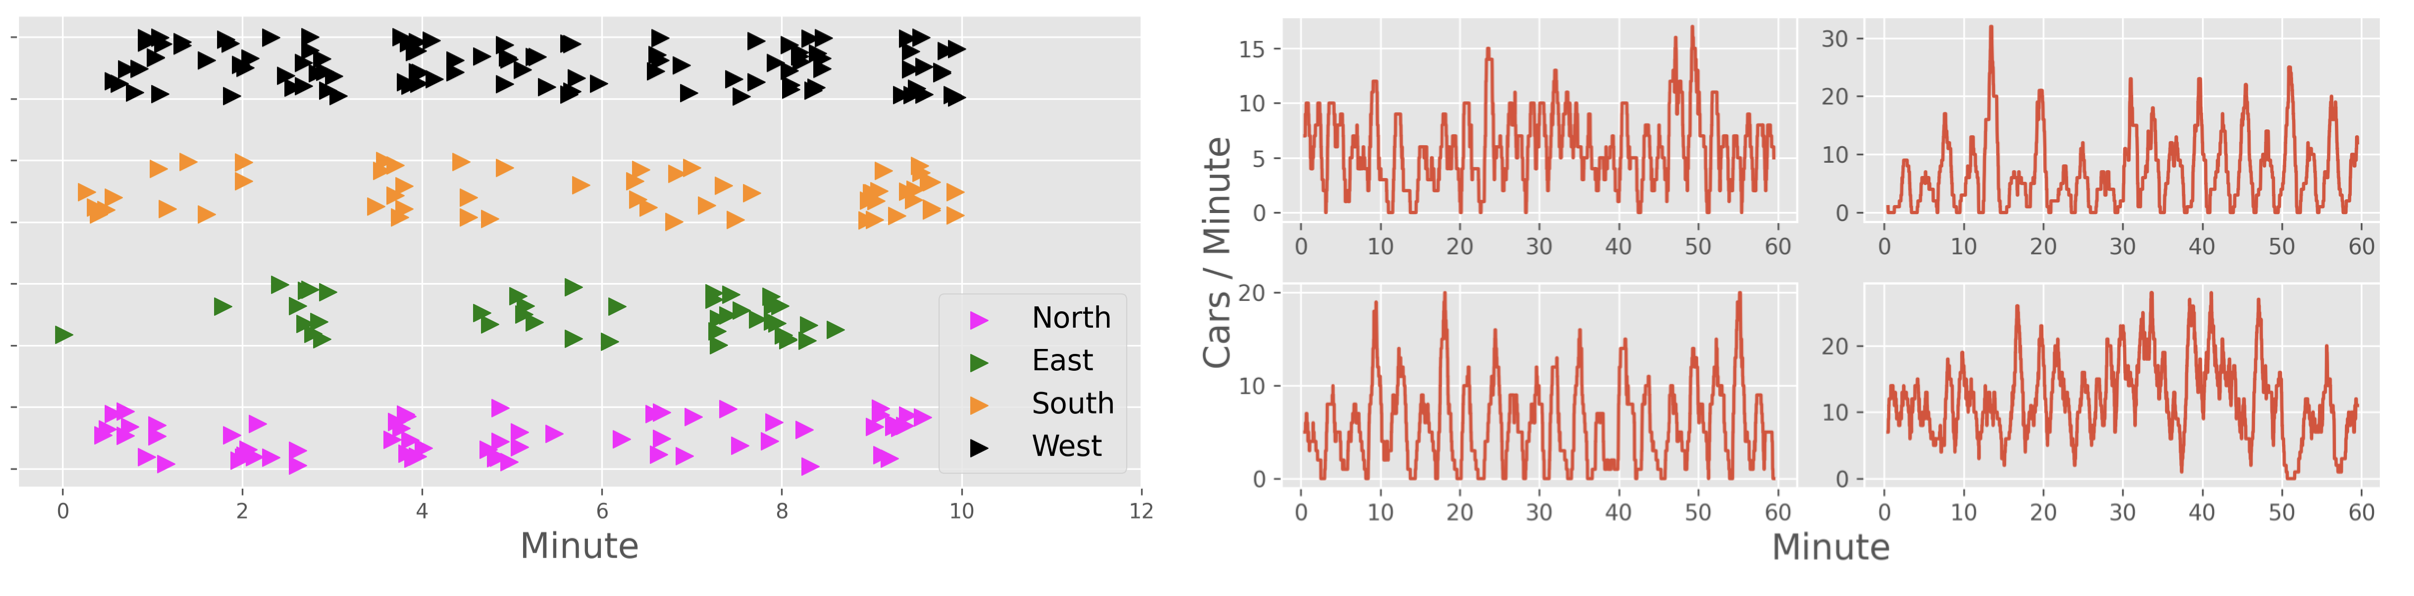
\includegraphics[width=1\linewidth]{images/related_work/atsc_representation.png}
    \caption{The left panel shows data from the first ten minutes of inflow on intersection Hangzhou 2, with every triangle indicating a vehicle. The right panel shows the rate of vehicles per minute. \cite{kanis2021deep}}
    \label{fig:atsc_clustering}
\end{figure}

To address these challenges, they introduce Reinforcement-Learning-Light (RLight)\cite{kanis2021deep}, a straightforward yet effective RL framework designed to exploit inductive biases specific to ATSC. Building on LIT's strengths, they enhance the state representation to accommodate clustered traffic data. In their approach, they distinguish between approaching and waiting vehicles, incorporating the mean speed and distance of the approaching cluster into the state representation. This method leverages the inherent structure of traffic clusters to keep the state representation concise and actionable. By using structured data sources such as ground sensors and GPS data, their approach bridges the gap between RL and real-world ATSC applications.

Notably, prior research has largely overlooked the modeling of yellow light in ATSC. While the problem has been traditionally framed as a standard MDP, they explore the potential of incorporating inductive biases that can skip redundant time steps during yellow lights, thus simplifying the reward signal and accelerating the learning process by approximately one-third.

Furthermore, there is no consensus in previous work regarding the safety and effectiveness of cyclic versus acyclic action spaces. They also investigate this difference, shedding light on the impact of allowing the agent to freely choose the optimal phase at each time step.

They evaluate their approach using real data from five intersections in Hangzhou, employing the CityFlow simulator \cite{zhang2019cityflow} unlike the simulator that I used in this work. To ensure the generalization of their method, they split the dataset into training, validation, and test sets. In their experiments, they compare RLight to a rule-based method known as Self-Organizing Traffic Lights (SOTL) \cite{cools2008selforganizing} in both multi-phase and two-phase settings. According to them they achieve outstanding results where RLight consistently outperforms state-of-the-art methods across all five intersections.

In summary, their contributions in this research are as follows:
\begin{itemize}
    \item Introduction of RLight, a straightforward RL framework that exploits inductive biases relevant to ATSC. Their cluster-aware state representation outperforms existing methods on the Hangzhou dataset.
    \item Proposal of reformulation of the MDP that eliminates redundant yellow light time steps, significantly expediting the learning process.
    \item Investigation of the performance difference between acyclic and cyclic phase transitions, offering valuable insights into the design of action spaces.
    \item Extension of the rule-based SOTL algorithm to work in an acyclic manner for multi-phase intersections.
\end{itemize}

According to them their single-agent approach demonstrates the capability to effectively control varying traffic densities, making it adaptable to unexpected real-world scenarios, including events, accidents, or unforeseen situations like a pandemic.

\subsection{RLight Agent Design}
\label{sec:rlight_agent_design}

Their RLight agent is based on the standard RL framework \cite{sutton2018reinforcement}. In the following sections, we will briefly describe how they formulate ATSC as an MDP and delve into the state and action representation, as well as the reward function. They consider scenarios where the agent controls a single intersection with \(J\) incoming lanes and \(I\) traffic light phases.

\subsection{Markov Decision Process}
\label{sec:mdp}

In ATSC problems, the modeling of the action rate has received limited attention in previous research. They consider two options based on the timestep rate of one simulation second per transition and a fixed yellow light period.

\textbf{MDP (Markov Decision Process):} In this approach, the agent selects an action at each simulation second, but actions during yellow light are ignored by the environment. This means the agent must learn that actions during yellow states have no impact on the final reward. Consequently, training effort is wasted on learning irrelevant state-action pairs, potentially introducing noise into the reward signal.

\textbf{SMDP (Semi-Markov Decision Process):} In this scheme, the agent only chooses actions when its decisions affect the environment, remaining inactive during yellow light. This can be seen as a Semi-Markov Decision Process (SMDP) \cite{sutton1999between}. The yellow period has a fixed length of \(\psi\) timesteps. When the agent switches to another phase at timestep \(\tau\), it receives cumulative discounted rewards during the yellow period, enhancing learning efficiency.

\subsubsection{State Representation}
\label{sec:state_representation}

The state representation is a vital aspect of ATSC. At each time step, the agent receives a quantitative representation of the environment, which they aim to make easily digestible while containing the necessary information for decision-making.

Starting with the number of vehicles and the current phase, as used in LIT \cite{zheng2019diagnosing}, they introduce:

\[
\boldsymbol{s}_t = [ \boldsymbol{w}_t^\intercal + \boldsymbol{a}_t^\intercal , \boldsymbol{p}_t^\intercal ] ,
\]

where \(\boldsymbol{w} + \boldsymbol{a} \in \mathbb{R}^J\) represents the total number of vehicles (waiting, \(w\), plus approaching, \(a\)) on each lane, and \(\boldsymbol{p}\) is the phase represented as a one-hot vector of size \(I\), where \(I\) and \(J\) are the number of phases and lanes, respectively.

However, this simple approach may lead to indistinguishable states, hindering learning. To address this, they explicitly separate waiting and approaching vehicles, catering to the fragmented distribution of urban traffic. Additionally, they incorporate the average speed and distance of approaching traffic to improve traffic anticipation, enabling earlier phase switches if a cluster moves faster or closer.

This enhanced state representation becomes:

\[
\boldsymbol{s}_t = [\boldsymbol{w}_t^\intercal, \boldsymbol{a}_t^\intercal, \boldsymbol{d}_t^\intercal, \boldsymbol{s}_t^\intercal, \boldsymbol{p}_t^\intercal],
\]

where \(\boldsymbol{w}\) represents the number of waiting vehicles, \(\boldsymbol{a}\) the number of approaching vehicles, \(\boldsymbol{d}\) is the average distance of approaching vehicles, \(\boldsymbol{s}\) is the average speed of approaching vehicles, and \(\boldsymbol{p}\) is the phase represented as a one-hot vector, with all values normalized. This method assumes that vehicles behave like steady convoys, leading to a state-space dimension of \(4 \times J + I\).

\subsubsection{Action Space} \label{rlight_action_space}
\label{sec:action_space}

At each timestep \(t\), the agent selects an action \(a_t\) from the available set of actions \(\mathcal{A} = \{1, \ldots, K\}\). They aim to provide the agent with maximum freedom to choose the most suitable action. They explore two options:

\textbf{Cyclic:} In this configuration, we use a predetermined phase sequence where the agent can either keep the current phase or switch to the next phase. The neural network outputs a value to indicate whether to switch or stay.

\textbf{Acyclic:} In the acyclic setup, the agent can freely choose the next phase, offering more flexible control. Here, the network outputs as many values as there are phases.

\subsubsection{Reward Function}
\label{sec:reward_function}

In ATSC, the agent receives a numerical reward \(r_t\) at each timestep, which is defined by the reward function. Their aim is to formulate a reward function that minimizes average travel time, assuming it as the primary objective.

Average travel time is challenging to compute in real-time, and using it directly as the reward signal would result in sparse and delayed rewards. Therefore, they employ a shaping reward based on the total queue length at the intersection \cite{zheng2019diagnosing}:

\[
\mathcal{R}(s) = - \sum_j w(s)_j t_j,
\]

where \(w_j\) is the queue length on lane \(j\) and \(j\) is the number of lanes. This shaping reward is proportionally related to the average travel time when speed changes are neglected.

\subsection{Self-Organizing Traffic Lights 2.0}
\label{sec:sotl_2.0}

In this section, we will discuss their adaptation for the rule-based Self-Organizing Traffic Lights (SOTL) algorithm to accommodate multi-phase settings. The original SOTL was primarily designed for two-phase settings, where the agent would switch to the next phase. However, in multi-phase intersections, the problem becomes more complex as multiple phases can exceed the threshold simultaneously. To address this, they introduce modifications to the algorithm.

In the original implementation, a key issue arises when transitioning to a multi-phase intersection. The resetting of a parameter, denoted as \(\kappa\), to zero no longer sufficiently conveys that vehicles have passed through a green phase. This is particularly problematic when multiple phases share lanes. If one phase turns green, the vehicles on the shared lane will pass through it, affecting \(\kappa\) for that phase. However, \(\kappa\) for other phases sharing the lane remains unaffected. As a result, the phase with the most cumulative waiting time is chosen, even if no vehicles are waiting for it. To overcome this, they introduce a new parameter, \(\rho\), which represents a set of counters to track vehicle integrals per lane over time. When a lane gets a green light, all corresponding counters are reset, ensuring that passed vehicles are removed from all relevant integrals.

In this extended SOTL algorithm, the phase with the maximum cumulative waiting time, denoted as \(\kappa\), is chosen. The algorithm's parameters include the current duration of the phase \(\phi_{\text{green}}\), the minimal phase duration \(\phi_{\text{min}}\), the number of vehicles within a specified distance from green lights \(v_{\text{vehicles}}^{\text{green}}\), a tunable parameter \(\mu\) that determines the number of vehicles needed to split a cluster, and the set of counters \(\rho\) corresponding to each phase \(\phi_i\).

\begin{algorithm}
\caption{SOTL Generalized to Multi-Phase Settings\cite{kanis2021deep}}
\label{alg:sotl_multi_phase}
\begin{algorithmic}
\State Initialize \(\kappa\) and \(\rho\) to 0
\For{\(t\) from 1 to \(T\)}
    \For{each lane \(j\)}
        \State \(\rho \mathrel{+}= \nu_j\)
    \EndFor
    \For{each phase \(i\)}
        \State Compute \(\kappa_i\) according to the integrals \(\rho\) and the phase duration \(\phi_i\)
    \EndFor
    \If{\(\phi_{\text{green}} > \phi_{\text{min}}\)}
        \State Determine the phase with the highest \(\kappa\)
        \State Choose the corresponding action
    \EndIf
\EndFor
\end{algorithmic}
\end{algorithm}

This extended algorithm ensures that the phase with the most waiting time is selected, while simultaneously addressing the issue of passed vehicles in multi-phase intersections. Importantly, the modified algorithm operates effectively in two-phase, four-approach settings, akin to the original SOTL method.


\section{Diagnosing Reinforcement Learning for Traffic Signal Control}
In this section, we discuss relevant study that was done for diagnosing some of the Reinforcement Learning algorithms for Traffic Signal Control. \cite{zheng2019diagnosing}. We will provide some brief overview of their work. Most of the formulas will be directly cited from their work to have understanding of the their interception of the Reinforcement Learning algorithms for Traffic Signal Control.

\subsection{Problem Formulation}

The problem of optimizing traffic signal control using RL is rooted in the definition of the RL environment. The state representation and the decision-making process play a crucial role in this context. The RL agent observes the environment, represented as a numerical state representation $s_t$, and makes decisions on whether to change the signal to the next phase or keep the current signal, denoted as $a_t$. This concept of a pre-defined signal phase order aligns with established practices in transportation engineering  ensuring driver expectations and safety considerations.

\subsubsection{Formal Problem Statement}

The core problem addressed in these studies can be formally defined as follows:

\textbf{Problem 1.} Given the state observations set $S$, action set $A$, and the reward function $R(s, a)$, the problem is to learn a policy $\pi(a|s)$ that maximizes the expected discounted return:

\[
G_t = R_{t+1} + \gamma R_{t+2} + \gamma^2 R_{t+3} + \ldots = \sum_{b=0}^{\infty} \gamma^b R_{t+b+1}
\]

Key components of this problem include state representations, action decisions, and reward structures.

\subsubsection{State, Action, and Reward}

The state representation typically includes information about the number of vehicles on each lane ($v_{j,t}$) and the current signal phase ($p_t$). The action is binary, where the signal can either change ($a_t = 1$) or remain the same ($a_t = 0$). The reward is defined as the summation of queue length over all lanes:

\[
R_t = -\sum_{j=1}^M q_{t, j}
\]

Here is a summary of the key notation used in these RL-based traffic signal control studies (Table 1).

\begin{table}[h]
\centering
\begin{tabular}{ll}
\textbf{Notation} & \textbf{Meaning} \\
$s$ & State \\
$a$ & Action \\
$R$ & Reward \\
$q_j$ & Queue length on lane $j$ \\
$v_j$ & Number of vehicles on lane $j$ \\
$p$ & Signal phase \\
$K$ & Number of signal phases \\
$M$ & Number of lanes \\
$N$ & Number of vehicles in the system \\
\end{tabular}
\end{table}

% \subsection{Objective}

% The primary objectives of the research in this area can be summarized as follows:

% \begin{itemize}
%     \item Find an RL algorithm to effectively address the traffic signal control problem.
%     \item Establish connections between RL algorithms and classic transportation theory, demonstrating the optimality of the RL approach.
%     \item Analyze the traits that make RL outperform other traditional methods in traffic signal control.
% \end{itemize}

% This review sets the stage for our proposed RL approach and its contributions to solving the traffic signal control problem.


% Hello there
% \subsection{Methodology}

% Several studies have delved into traffic signal control problems using RL. A key development in this field is the Light-IntellighT (LIT) method, which is designed to address the traffic signal control problem. LIT adopts a specific state and reward design, aligning with the approach outlined in Section 3.2.

% \subsubsection{Deep Q-Network}

% LIT leverages the Deep Q-Network (DQN) \cite{intellilight-rl-traffic-light} to seek actions that maximize long-term rewards. The Bellman Equation \cite{sutton1999between} serves as a fundamental principle in this approach:

% \[
% Q(s_t, a_t) = R(s_t, a_t) + \gamma \max Q(s_{t+1}, a_{t+1})
% \]

% The use of DQN, as illustrated in Figure 2, demonstrates the effective use of features such as vehicle numbers and phase indicators.

% \subsubsection{Classic Transportation Theory}

% Before delving into RL-based traffic signal control algorithms, it's important to consider traditional transportation theory. The optimization of traffic signal control from a transportation research perspective focuses on minimizing total travel time under specific traffic conditions.

% The mathematical expression for this optimization problem involves constraints related to green phase allocation and traffic flow:

% \[
% \begin{array}{ll}
% \text{minimize} & \sum_{j=1}^M T_j \\
% \text{subject to} & g^{\text{min}} \leq g_k \leq g^{\max} \\
% & \frac{g_j}{C} \geq \frac{f_{in, j}}{u_{sat, j}}, \quad j=1,2,3, \ldots, M
% \end{array}
% \]

% The constraints ensure appropriate green phase allocation and traffic flow considerations. This traditional transportation approach lays the foundation for understanding the traffic signal control problem from a different perspective.

% \subsubsection{Connecting RL with Transportation Theory}

% This section aims to build connections between the RL algorithm and transportation methods. It highlights the equivalence between using queue length as a reward function in RL and optimizing travel time in transportation methods. Additionally, the use of the number of vehicles on each lane ($v_j$) and the current phase ($p$) as the only state features is discussed, emphasizing their importance in understanding system dynamics.

% \subsubsection{Analysis of Traits of RL Approach}

% The analysis of RL's traits that enable it to outperform traditional methods is another critical aspect of these studies. These traits include:

% \begin{itemize}
%     \item Online learning: RL algorithms adapt in real-time based on feedback from the environment, learning from mistakes.
%     \item Sampling guidance: RL employs experience to make guided decisions, improving convergence and reward.
%     \item Forecast: RL predicts future rewards through the Bellman equation, which enables actions for long-term rewards.
% \end{itemize}

% These traits distinguish RL as a powerful approach in traffic signal control.

% In the following sections, we present our proposed RL approach, building upon the insights gained from the related work.
